\documentclass[12pt, twoside]{article}
\documentclass[12pt, twoside]{article}
\usepackage[letterpaper, margin=1in, headsep=0.2in]{geometry}
\setlength{\headheight}{0.6in}
%\usepackage[english]{babel}
\usepackage[utf8]{inputenc}
\usepackage{microtype}
\usepackage{amsmath}
\usepackage{amssymb}
%\usepackage{amsfonts}
\usepackage{siunitx} %units in math. eg 20\milli\meter
\usepackage{yhmath} % for arcs, overparenth command
\usepackage{tikz} %graphics
\usetikzlibrary{quotes, angles}
\usepackage{graphicx} %consider setting \graphicspath{{images/}}
\usepackage{parskip} %no paragraph indent
\usepackage{enumitem}
\usepackage{multicol}
\usepackage{venndiagram}

\usepackage{fancyhdr}
\pagestyle{fancy}
\fancyhf{}
\renewcommand{\headrulewidth}{0pt} % disable the underline of the header
\raggedbottom
\hfuzz=2mm %suppresses overfull box warnings

\usepackage{hyperref}
\usepackage{float}

\title{Algebra 2}
\author{Chris Huson}
\date{November 2024}

\fancyhead[LE]{\thepage}
\fancyhead[RO]{\thepage \\ First and last name: \hspace{2.5cm} \,\\ Section: \hspace{2.5cm} \,}
\fancyhead[LO]{BECA / Huson / Precalculus: 3. Complex numbers \\* 13 December 2024}

\begin{document}

\subsubsection*{3.19 Test: Rational exponents and complex numbers \hfill A2.A.APR.6}
\begin{enumerate}[itemsep=0.5cm]
\subsubsection*{A2-APR.1 Perform operations with polynomials}
% Problem 1
\item Find the sum in standard form:
\[
(- 3x^3 + 2x^2 + 7x - 4) + (5x^3 + x^2 - 3x + 9).
\] \vspace{4cm}

% Problem 2
\item Find the difference \(f(x) - g(x)\) as a polynomial in standard form, given:
\[
f(x) = x^4 - 3x^3 - 3x^2 - 2x + 5 \quad \text{and} \quad g(x) = 2x^4 - x^3 + 2x + 5.
\] \vspace{4cm}

\item Select each correct equation.
\begin{multicols}{2}
    \begin{enumerate}
    \item $x^2 + 14 = x^2 + 7^2$
    \item $x^2 + 49 = (x-7)(x+7)$
    \item $x^2 - 49 = (x-7)(x+7)$
    \item $x^2 + 14x + 49 = (x-7)^2$
    \item $x^2 - 14x + 49 = (x+7)^2$
    \item $x^2 - 14x + 49 = (x-7)^2$
    \end{enumerate}
\end{multicols}
        
\item Which equations represent correct polynomial identities?
\begin{multicols}{2}
    \begin{enumerate}
    \item \(x^3 - y^3 = (x - y)^3\)
    \item \(x^3 - y^3 = (x + y)(x^2 + xy + y^2)\)
    \item \(x^3 + y^3 = (x + y)(x^2 - xy + y^2)\)
    \item \(x^3 + y^3 = (x - y)(x^2 - xy + y^2)\)
\end{enumerate}
\end{multicols}
    
\newpage
\subsubsection*{A2-F.IF.7a Graph linear and quadratic functions, show key features}
\item One equation of a system is graphed. 
\begin{enumerate}
    \item Graph the second equation, labeling the intersections as ordered pairs.
    \item Find the value of the leading coefficient $a$ of the quadratic equation.
\end{enumerate}
\begin{multicols}{2}
    \hspace{1cm} $y = ax^2 + 4x + 5$ \\
    \columnbreak
    $x - y = 7$
    \end{multicols}
     \vspace{3cm}

  \begin{center}
  \begin{tikzpicture}[scale=.635]
    \draw [help lines] (-10,-10) grid (10,10);
    \draw [thick, ->] (-10.2,0) -- (10.4,0) node [below right] {$x$};
    \draw [thick, ->] (0,-10.2)--(0,10.4) node [left] {$y$};
    \draw[thick, <->,smooth, domain=-2.15:4.8] plot (\x, {-1.5*(\x)^2 + 4*\x + 5});
  \end{tikzpicture}
  \end{center}
  

\newpage
\subsubsection*{A2-A.APR.3 Identify zeros of polynomials given suitable factorizations}
\item Write down the solutions to the equation $(x - 7)(4x + 3)(x - 2) = 0$. \vspace{2cm} 

\item The polynomial $p$ is a function of $x$. The graph of $p$ has zeros at $0$, $3$, $\frac{5}{3}$, and $-7$. Select $\bf{all}$ the expressions that could represent $p$. \vspace{0.25cm}
    \begin{multicols}{2}
    \begin{enumerate}
        \item $(x-3)(x-\frac{5}{3})(x+7)$
        \item $x(x+3)(5x-3)(x+7)$
        \item $3(x+3)(x-\frac{5}{3})(x+7)$
        \item $3x(x-3)(x-\frac{5}{3})(x+7)^2$
        \item $(x-3)(x+\frac{5}{3})(x-7)$
        \item $x(x-3)(3x-5)(x+7)$
        \item $3(x-3)(x-\frac{5}{3})(x-7)$
        \item $3x(x-3)(x-\frac{3}{5})(x+7)^2$
    \end{enumerate}
    \end{multicols}

\subsubsection*{A2-A.REI.2 Solve rational and radical equation, identify extraneous solutions}
\item Square both sides of the equation and solve for $x$.
    \begin{multicols}{2}
    \begin{enumerate}[itemsep=0.5cm]
        \item  $\sqrt{x + 9}=4$
        \item Check your solution.
    \end{enumerate}
    \end{multicols} \vspace{3cm}

\item Solve for $x$ and check.
    \begin{multicols}{2}
    \begin{enumerate}[itemsep=0.5cm]
        \item  $\sqrt{5x+16} + 5 = 14$
        \item Check your solution.
    \end{enumerate}
    \end{multicols} \vspace{3cm}

\newpage
\item Select the expression that is equivalent to $\displaystyle \frac{5x^2 + 2x - 30}{x - 3}$ for $x \neq 3$.
    \begin{enumerate}
        \item $\displaystyle 5x - 13 + \frac{16}{x - 3}$
        \item $\displaystyle 5x + 17 + \frac{21}{x - 3}$
        \item $\displaystyle 5x - 13 + \frac{8}{x - 3}$
        \item $\displaystyle 5x + 17 + \frac{15}{x - 3}$
    \end{enumerate}
    \vspace{2cm}

\item Solve for $x$. $\displaystyle \frac{2}{x+3} = \frac{x+1}{x}$ \vspace{5cm}


\subsubsection*{A2-F.BF.2 Write arithmetic and geometric sequences with recursive formulas}
\item Write a recursive definition of the sequence $a_1 = 0.25$, $a_2 = 0.75$, $a_3 = 1.25$, $a_4 = 1.75, \ldots$ \vspace{1cm}

\item Write a recursive definition of the geometric sequence $b$. \\[0.5cm]
\renewcommand{\arraystretch}{1.5}
\begin{tabular}{|c|c|}
\hline
$n$ & $b_n$ \\
\hline
$1$ & $-1$ \\
$2$ & $5$ \\
$3$ & $-25$ \\
\hline
\end{tabular} \vspace{1cm}

\newpage 
\subsubsection*{A2-F.IF.7c Graph polynomials, identify zeros, end behavior}
\item Below is a graph of the polynomial $g(x)$. 
\begin{multicols}{2}
    \begin{enumerate}[itemsep=1cm]
        \item Is the leading coefficient positive or negative?
        \item Which of the following could be its equation?
        \begin{enumerate}
            \item $g(x) = -(x+1)(x-3)(x-1)^2$
            \item $g(x) = -(x-1)(x-3)(x+1)^2$
            \item $g(x) = -(x+1)(x+3)(x-1)^2$
            \item $g(x) = -(x-1)(x+3)(x+1)^2$
        \end{enumerate} \vspace{1cm} \;
    \end{enumerate}

    \columnbreak
    \begin{tikzpicture}[xscale=0.7, yscale=0.7]
        \draw[lightgray,very thin] (-4,-3) grid (4,5);
        \draw [thick, ->] (-4.5,0) -- (4.5,0) node [above] {$x$};
        \draw [thick, ->] (0,-3)--(0,5.5) node [right] {$y$};
        \foreach \x in {-4,-3,-2,-1,0,1,2,3,4} \draw (\x cm,5pt) -- (\x cm,-5pt) node[below] {$\x$};
        %\foreach \y in {-10,10} \draw (5pt,\y cm) -- (-5pt,\y cm) node[left] {$\y$};
        \draw [thick, <->,smooth,samples=50,domain=-1.15:3.15] plot(\x,{-(\x+1)*(\x-3)*(\x-1)*(\x-1)});
    \end{tikzpicture}
\end{multicols}

\item The graph of the polynomial $-x^{4}+3x^{3}-x^{2}-3x+2$ is shown. 
\begin{multicols}{2}
    \begin{enumerate}[itemsep=1cm]
        \item What is the degree of the function?
        \item What are the zeros of the function?
        \item Which factor has a multiplicity of 2?
        \item Write down the $y$-intercept as an ordered pair.
        \item Three points are marked on the graph, $p$, $q$, and $r$. Which one is a local maximum?
    \end{enumerate} \vspace{1cm} \;

    \columnbreak

    \begin{tikzpicture}[xscale=0.7, yscale=0.8]
        \draw[lightgray,very thin] (-4,-5) grid (4,5);
        \draw [thick, ->] (-4.2,0) -- (4.4,0) node [above] {$x$};
        \draw [thick, ->] (0,-5.2)--(0,5.5) node [right] {$y$};
        \foreach \x in {-4,4} \draw (\x cm,5pt) -- (\x cm,-5pt) node[below] {$\x$};
        \draw (5pt,5 cm) -- (-5pt,5 cm) node[left] {$5$};
        \draw [thick, <->,smooth,samples=50,domain=-1.3:2.6] plot(\x,{-(\x+1)*(\x-2)*(\x-1)*(\x-1)});
        \filldraw [black] (-0.44, 2.83) circle (2.5pt) node[above left]{$p$};
        \filldraw [black] (-1, 0) circle (2.5pt) node[above right]{$q$};
        \filldraw [black] (1.7, 0.4) circle (2.5pt) node[above]{$r$};
    \end{tikzpicture}
\end{multicols}

\newpage
\item The graph of the function $f(x) = x^3 - 3x^2 - 10x + 24$ is shown. Write the function in factored form. 
    \begin{flushright}
    \begin{tikzpicture}[xscale=1, yscale=0.25]
        \draw [thick, ->] (-4.2,0) -- (5,0) node [above] {$x$};
        \draw [thick, ->] (0,-8.2)--(0,10) node [right] {$y$};
        \foreach \x in {-3,...,4} \draw (\x cm,12pt) -- (\x cm,-12pt) node[below] {$\x$};
        %\foreach \y in {-8,-6,4,8} \draw (3pt,\y cm) -- (-3pt,\y cm) node[left] {$\y$};
        \draw [thick, <->,smooth,samples=20,domain=-3.6:4.6] plot(\x,{0.3*(\x-2)*(\x-4)*(\x+3)});
    \end{tikzpicture}
    \end{flushright}

\item Let $j(x)= (x+4)(x+1)(x-4)^2$ be a polynomial function. 
    \begin{center}
    \begin{tikzpicture}[xscale=0.7, yscale=0.7]
        \draw [thick, ->] (-7.2,0) -- (7.5,0) node [above] {$x$};
        \draw [thick, ->] (0,-5.2)--(0,6.5) node [right] {$y$};
        \foreach \x in {-7,...,7} \draw (\x cm,5pt) -- (\x cm,-5pt);
    \end{tikzpicture}
    \end{center}
    \begin{enumerate}[itemsep=0.25cm]
        \item Sketch a graph of the function. Label the $x$-intercepts.
        \item Find the value of the $y$-intercept and mark it on the graph. \vspace{1cm}
        \item Identify the end behavior of the function.
            \begin{multicols}{2}
            \begin{enumerate}
                \item As $x \to +\infty$, $y \to +\infty$; \\ 
                as $x \to -\infty$, $y \to -\infty$
                \item As $x \to +\infty$, $y \to -\infty$; \\
                as $x \to -\infty$, $y \to +\infty$
                \item As $x \to +\infty$, $y \to +\infty$; \\
                as $x \to -\infty$, $y \to +\infty$
                \item As $x \to +\infty$, $y \to -\infty$; \\
                as $x \to -\infty$, $y \to -\infty$        
            \end{enumerate}
            \end{multicols}
    \end{enumerate}

\newpage

\subsubsection*{A2.N.CN.2 Apply the properties of complex numbers}
\item If \((6 - ki)^2 = 27 - 36i\), the value of \(k\) is
\begin{enumerate}
    \item \(-36\)
    \item \(-3\)
    \item \(3\)
    \item \(6\)
\end{enumerate} \vspace{1cm}

\item Does the equation $x^2 - 4x + 13 = 0$ have imaginary solutions? Justify your answer.

\newpage
\subsubsection*{HSN.RN.2 Expressions with radicals and rational exponents}
\item Simplify each radical expression, using complex numbers as necessary.
    \begin{multicols}{2}
    \begin{enumerate}[itemsep=0.5cm]
        \item $\sqrt{64}=$
        \item $\sqrt{27}=$
        \item $\sqrt{-9}=$
        \item $\displaystyle \frac{\sqrt{-50}}{\sqrt{2}}=$
    \end{enumerate}
    \end{multicols} \vspace{1cm}
    
\item Simplify each expression.
    \begin{multicols}{2}
    \begin{enumerate}[itemsep=0.5cm]
        \item $\displaystyle 125^{\frac{2}{3}} =$
        \item $\left( \sqrt[3]{\frac{8}{27}} \right)^{2} =$
    \end{enumerate}
    \end{multicols} \vspace{2cm}

    
\item Rewrite each expression as a fractional exponent in simplest terms. $x>0$
    \begin{multicols}{2}
      \begin{enumerate}[itemsep=1cm]
          \item $\sqrt[3]{7} =$
          \item $\displaystyle \frac{1}{\sqrt[3]{5}}=$
          \item $\sqrt[2]{x^4} =$
          \item $\displaystyle \frac{1}{(\sqrt[3]{x})^2}=$
      \end{enumerate}
      \end{multicols} \vspace{1cm}
  
\item Rewrite each expression with fractional exponent as a radical.
    \begin{multicols}{2}
      \begin{enumerate}[itemsep=1cm]
        \item $\displaystyle 5^{\frac{1}{4}}=$
        \item $\displaystyle 5^{-\frac{1}{3}}=$
        \item $\displaystyle x^{\frac{2}{5}}=$
        \item $\displaystyle x^{-\frac{1}{3}}=$
      \end{enumerate}
      \end{multicols}
       
\end{enumerate}
\end{document}